\subsection{Tempo de vida a partir das oscilações de energia}
Na análise anterior, foi examinada a perda de elétrons devido a flutuações anormais nas amplitudes das oscilações radiais. A perda de elétrons de um feixe também irá ocorrer quando flutuações anormais nas oscilações de energia resultarem em excursões de energia tão grandes que não possam mais ser contidas na curva separatriz determinada pelo sistema de RF.

Na \autoref{sec:3.6} foi visto que as oscilações de energia correspondem ao movimento de uma partícula ideal em uma curva potencial, onde uma das paredes é um potencial em forma de "montanha" com altura limitada. A situação foi descrita na \autoref{fig:fig36}(b) e uma parte está redesenhada na \autoref{fig:fig48}(a). A coordenada horizontal é o deslocamento de tempo $\tau$ associado às oscilações de energia e a coordenada vertical é a "energia potencial" fictícia da oscilação. A "energia cinética" correspondente é
\begin{align}
	\frac{1}{2}\left(\frac{d\tau}{dt}\right)^2 = \frac{\alpha^2}{2}\left(\frac{\epsilon}{E_0}\right)^2\label{eq:5.131}
\end{align}
onde $\epsilon$ é o desvio de energia instantâneo da oscilação de energia real.

\begin{figure}[!htb]
	\centering
	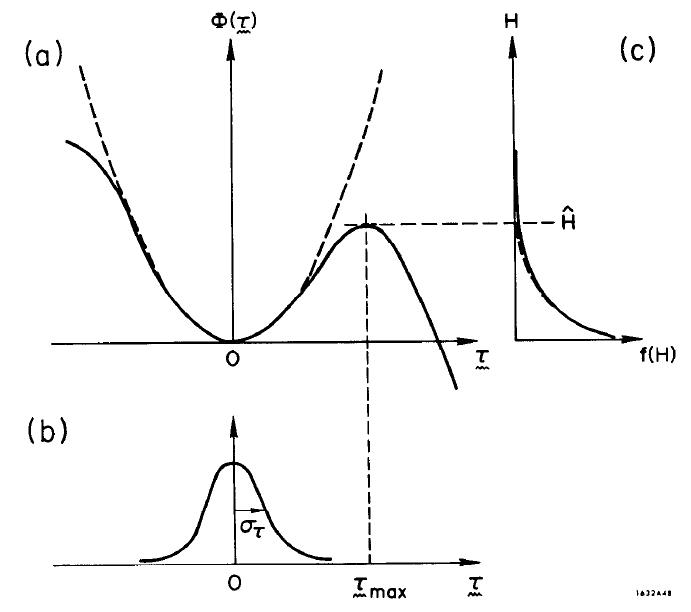
\includegraphics[width=0.6\linewidth]{./Figuras/fig48.jpeg}
	\caption{\textit{Spread} quântico nas oscilações de energia. Retirado de \cite{sands1970physics}.}
	\label{fig:fig48}
\end{figure}

Suponha que $H$ represente a "oscilação de energia total" -- isto é, a soma da "energia potencial" e da "energia cinética" da equação \eqref{eq:5.131} --
\begin{align}
	H = \Phi(\tau) + \frac{\alpha^2}{2}\left(\frac{\epsilon}{E_0}\right)^2
\end{align}
($\Phi$ é zero no fundo da curva potencial). Durante a oscilação de um elétron em particular, a "energia potencial" alcançada no $\tau$ máximo é igual a $H$. E a "energia cinética" de pico -- a qual ocorre quando o elétron passa $\tau=0$ -- também é igual a $H$, então
\begin{align}
	H = \frac{\alpha^2}{2}\left(\frac{\hat{\epsilon}}{E_0}\right)^2
\end{align}
onde $\hat{\epsilon}$ é o valor de pico de $\epsilon$ durante sua oscilação. O elétron está contido numa oscilação de energia estável se $H$ é menor que $\Phi_{max}$, a altura máxima da curva potencial (veja a \autoref{sec:3.6}). Do contrário, ele será perdido.
 Na \autoref{sec:5.2} e na \autoref{sec:5.3}, foram examinadas as oscilações de energia induzidas quanticamente seguindo a suposição de que essas eram idealmente lineares -- as quais corresponderiam à função potencial parabólica indicada pela linha tracejada na \autoref{fig:fig48}(a). Considerando estas suposições, a distribuição do deslocamento de tempo em um \textit{bunch} de elétrons armazenado seria a função Gaussiana desenhada na \autoref{fig:fig48}(b) -- cujo desvio padrão $\sigma_\tau$ foi avaliado na \autoref{sec:5.4}.
 
Também foi visto que as flutuações de energia levam a uma distribuição exponencial no quadrado da amplitude das oscilações de energia -- como foi descrito pela equação \eqref{eq:5.61}. A variável $W$ utilizada é apenas o quadrado da amplitude (da oscilação em $\epsilon$) e, portanto, proporcional a "energia total" $H$. De fato,
\begin{align}
	H = \frac{\alpha^2}{2E_0^2}W
\end{align}
Sendo assim, segue que a distribuição em $H$ para os elétrons armazenados em um \textit{bunch} também é exponencial. Mais especificamente, seja $f(H)dH$ a representação do número de elétrons com "energias totais de oscilação" entre $H$ e $H+dH$, pela equação \eqref{eq:5.62} é direto que
\begin{align}
	f(H)dH = \frac{N}{\mean{H}}\ e^{-H/\mean{H}}
\end{align}
onde
\begin{align}
	\mean{H} = \frac{\alpha^2}{2E_0^2}\mean{W} = \frac{\alpha^2}{E_0^2}\sigma_\epsilon^2
\end{align}
Esta distribuição das oscilações de energia é mostrada na \autoref{fig:fig48}(c).

Evidentemente, a situação real deve ser diferente. Qualquer elétron cujo deslocamento de tempo exceda $\tau_{max}$, o valor de $\tau$ no topo da montanha da curva real de potencial -- ou, de forma equivalente, um elétron cuja "oscilação de energia" $H$ exceda $\Phi_{max}$ -- será perdido do \textit{bunch}. Como foi visto na \autoref{sec:5.7} para as oscilações radiais, deve-se esperar que as distribuições reais irão a zero em $\tau_{max}$ -- e, portanto, em $H = \hat{H} = \Phi_{max}$. E então existirá uma perda de elétrons contínua devido à difusão para fora da cauda da distribuição.

A situação aqui é similar a que foi discutida na \autoref{sec:5.7}, onde a correspondência seria o súbito truncamento em $\tau_{max}$ da curva potencial parabólica. A curvatura suave do potencial máximo terá um efeito diferente no comportamento da distribuição de elétrons próximos ao limite da distribuição. No entanto, enquanto $\tau_{max} >> \sigma_\tau$, a taxa de perda de elétrons pode ser estimada da mesma forma em ambas as situações.

Sem repetir o raciocínio, pode-se escrever o resultado correspondente à equação \eqref{eq:5.127} para o caso das oscilações de energia:
\begin{align}
	\tau_q = \frac{\tau_\epsilon}{2}\frac{e^{\zeta}}{\zeta}
\end{align}
onde
\begin{align}
	\zeta = \frac{\hat{H}}{\mean{H}} = \frac{\Phi_{max}}{\mean{H}}
\end{align}
A altura $\Phi_{max}$ do potencial máximo pode ser avaliada pela integração da equação \eqref{eq:3.53} -- ou, para um tensão de RF senoidal, utilizando a equação \eqref{eq:3.58}.

O potencial $\Phi_{max}$ foi introduzido a fim de obter-se a magnitude da "abertura" das oscilações de energia. Ele está relacionado com o máximo desvio de energia aceitável $\epsilon_{max}$ -- veja a equação \eqref{eq:3.57} --
\begin{align}
	\Phi_{max} = \frac{\alpha^2}{2}\frac{\epsilon_{max}}{E_0}
\end{align}
Então $\zeta$ tem uma forma conceitualmente simples:
\begin{align}
	\zeta = \frac{\epsilon_{max}^2}{2 \sigma_\epsilon^2}
\end{align}

O potencial $\Phi_{max}$ e, portanto, o número $\zeta$ dependem da magnitude da tensão de RF, a qual precisa sempre ser suficientemente grande para resultar em um tempo de vida maior que o tempo de armazenamento desejado do feixe. Tipicamente, $\zeta$ deve ser em torno de 18 ou mais, fazendo necessário que $(\epsilon_{max}/\sigma_\epsilon)$ seja em torno de 6.

Para o caso particular (mas muito comum) de um anel de armazenamento com campo guia isomagnético e uma tensão de RF senoidal, o parâmetro $\zeta$ pode ser expresso em termos de parâmetros do anel. Juntando resultados obtidos anteriormente em outras seções para $\epsilon_{max}$ e $\sigma_\epsilon$, pode-se mostrar que
\begin{align}
	\zeta = \frac{J_\epsilon E_0}{\alpha k E_1}F(q)\ \ (isomag.)
\end{align}
onde $E_1$ é a constante com dimensões de energia:
\begin{align}
	E_1 = \frac{3 mc C_q}{2r_e} = \frac{55\sqrt{3}}{64} \frac{\hslash c}{r_e} \approx 1.08 \times 10^8\ eV
\end{align}
e $F(q)$ é a função de aceitância em energia definida na equação \eqref{eq:3.60} e mostrada na \autoref{fig:fig38}. O parâmetro $q$ é a sobretensão de RF -- mais exatamente, a relação entre a tensão de pico de RF e a perda de energia em uma volta. Para grandes sobretensões, $F(q)$ é aproximadamente $(2q-\pi)$ e o tempo de vida quântico aumenta exponencialmente com o aumento da tensão de RF.

Note que em um anel de armazenamento com um dado campo guia (isto é, com $\alpha$, $J_\epsilon$, $\tau_\epsilon$ e $E_0$ fixos) a sobretensão necessária para qualquer tempo de vida quântico em particular (isto é, para um $\zeta$ específico) depende do número harmônico $k$ e do sistema de RF. Para grandes números harmônicos, a sobretensão necessária varia em torno de $\sqrt{k}$. 